\documentclass{article}
\usepackage{booktabs}
\usepackage{amsmath,amssymb}
\usepackage{graphicx}
\usepackage{hyperref}
\usepackage[preprint]{icml2027}
\usepackage{colortbl}
\definecolor{TableInk}{HTML}{393B3C}
\definecolor{TableCream}{HTML}{F5EEE5}
\definecolor{TableBlue}{HTML}{E1EAF7}
\definecolor{TableGreen}{HTML}{E7EFDB}
\definecolor{TableOrange}{HTML}{F9E8D8}
\definecolor{TableGold}{HTML}{FBF0C8}
\newcommand{\paperTableStyle}{%
  \arrayrulecolor{TableInk}%
  \setlength{\heavyrulewidth}{0.70pt}%
  \setlength{\lightrulewidth}{0.40pt}%
  \setlength{\aboverulesep}{0pt}%
  \setlength{\belowrulesep}{0pt}%
  \renewcommand{\arraystretch}{1.12}%
}
\AddToHook{env/table/begin}{\paperTableStyle}
\AddToHook{env/table*/begin}{\paperTableStyle}
\newcommand{\paperHeader}{\rowcolor{TableCream}}
\newcommand{\paperHead}[1]{\textbf{#1}}


\icmltitlerunning{SPRINT: Feasible-Set-First Neural MIS Under a 200 ms Deadline}

\begin{document}
\twocolumn[
\icmltitle{SPRINT: Feasible-Set-First Neural Search for Maximum Independent Set Under a 200-Millisecond Deadline}
\begin{icmlauthorlist}
\icmlauthor{Han Zeng}{jnu}
\icmlauthor{Xin Zhang}{jnu}
\end{icmlauthorlist}
\icmlaffiliation{jnu}{Jiangnan University}
\icmlcorrespondingauthor{Xin Zhang}{zhangxin@jiangnan.edu.cn}
\icmlkeywords{maximum independent set, neural combinatorial optimization, GPU execution, anytime algorithms}
\vskip 0.3in
]

\printAffiliationsAndNotice{}

\begin{abstract}
A deadline-constrained solver should be judged by what it has delivered, not by what it would score with more time. We make delivery the metric on maximum independent set, where every delivered set is checkable against the input edges, and we hold it fixed across four graph families, four deadlines from 50 to 500~ms, and every measured neural, heuristic and exact solver. SPRINT, the solver family we introduce, answers a deadline with two routes. Its constructive route, SPRINT-C, publishes a greedy maximal set before the network is called and spends the rest of the budget on a learned-ranked exchange and clique-bound search; at 200~ms it delivers the largest mean set of any measured solver on all four families (20.1150, 42.4417, 44.3438 and 370.1250 vertices, ahead of resident OnlineMIS by 0.03, 0.68, 1.62 and 6.54), and on RB-[200--300] it reaches all 3,000 verified optima at every budget with one frozen checkpoint. Its speculative route, SPRINT-S, keeps 200 particles on the GPU: CUDA Graph replay and policy compilation raise executed updates in 200~ms from 82.9 to 348.6, adding 0.3320 vertices at unchanged per-step quality, and a midpoint decode makes the eventually scored set available 87.6~ms before the terminal one. What a deadline rewards is the decision to hold and publish a feasible set; the appendix isolates the smaller, family-dependent share that learned ordering contributes.
\end{abstract}

\section{Introduction}

A maximum independent set (MIS) selects assignments no two of which are incompatible, and a delivered set can be checked edge by edge against the input. That makes MIS a clean testbed: the answer names the vertices, so a caller can use it the moment it arrives. A solver that has found a large independent set may still be useless to a caller that needs the answer now. On 1,000 large RB graphs under a 50~ms budget, our solver holds a feasible set on the host in all 3,000 runs, yet 475 calls still return after that deadline. Neural MIS solvers are usually scored on objective value after a fixed number of steps or a fixed wall-clock slice, and neither number says when a feasible set became readable. We take delivery as the unit of measurement. Each candidate set is copied to a host archive and timestamped; the score at deadline \(B\) is the largest set in the archive at \(B\); the solver's return time is recorded separately. The archive stores vertices, so every scored set is re-checked against the input edges after timing.

This rule exposes a choice that objective-at-return hides: what the network should do with its budget. We study SPRINT, a solver family with two routes to an answer. SPRINT-S, the speculative route, uses a particle policy built on regularized Langevin dynamics \citep{feng2025regularized}, which updates many binary states in parallel. Those states may contain adjacent vertices, so each publication must first be decoded into an independent set, and every decode competes with search. SPRINT-C, the constructive route, instead builds a maximal independent set, publishes it, and calls the network once to rank vertices for exchanges and branch search. The designs answer different questions: whether another decode pays for itself, and whether learned guidance improves on a cheap structural order.

Answering either question requires holding everything but the factor of interest fixed. We give native OnlineMIS an in-memory entry point and the same archive, so it can publish during its call instead of only on exit, and inside otherwise identical SPRINT-C search we replace the neural ranking with degree ranking, charging each for its own inference. The same graph--seed pairs are solved at four deadlines from 50 to 500~ms.

\textbf{SPRINT-C wins at 200~ms on every family.} It exceeds resident OnlineMIS by 0.03, 0.68, 1.62 and 6.54 vertices, and every paired interval excludes zero (Table~\ref{tab:external-deadline}); on RB-[200--300] it reaches all 3,000 verified optima at all four budgets with one frozen checkpoint. \textbf{Execution carries the particle route.} CUDA Graph replay and compilation raise executed updates in 200~ms from 82.9 to 348.6 and add 0.3320 vertices at unchanged per-step quality, while a midpoint decode leaves mean size unchanged and makes the eventually scored set available 87.6~ms earlier. \textbf{Delivery, not the refinement order, is what a deadline rewards.} Degree ordering alone recovers most of the constructive gap, and Appendix~\ref{app:gain-sources} quantifies the ranking's share; Figure~\ref{fig:intro-evidence} traces the same comparison as elapsed time and breaks the 200~ms gains down by comparator.

We contribute (i) a delivery protocol for deadline-constrained combinatorial search, with a host archive, per-instance timestamps and paired controls at four budgets; (ii) SPRINT, whose constructive route holds and publishes a feasible set from the first millisecond and whose speculative route converts faster transitions into extra proposals; and (iii) a controlled decomposition of the delivered size into the part explained by construction and publication and the part explained by learned ordering, on four graph families and 14 register instances.

\begin{figure*}[t]
\centering
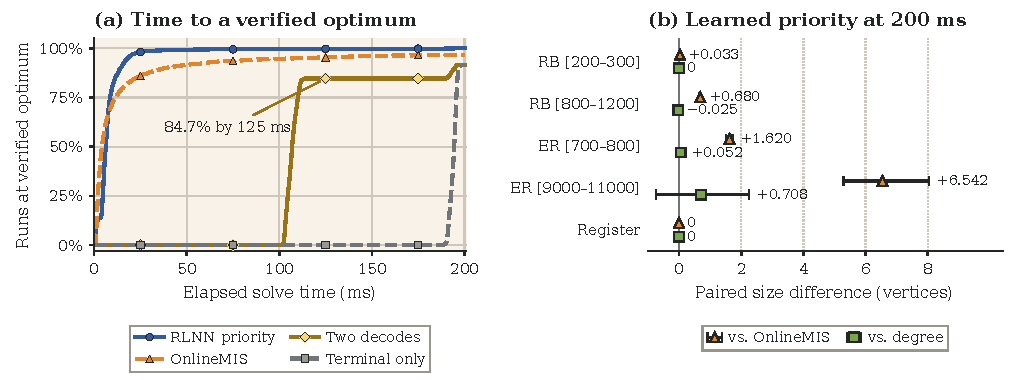
\includegraphics[width=1.0\textwidth]{figures/intro_evidence.pdf}
\caption{\textbf{Delivery timing and the effect of learning.}
(a) Curves show the share of 3,000 small RB graph--seed pairs with an offline-verified optimum already on the host. The particle clock starts at per-graph buffer loading and the resident clock at the host edge list. By 125~ms, two decodes deliver 2,540 optima and terminal-only decoding delivers none. Both reach 2,750 by 200~ms.
(b) Points show learned priority minus each comparator in mean delivered size at 200~ms. Whiskers give pointwise 95\% graph-bootstrap intervals. Small ER uses the single-core interleaved repeat. All three methods tie on every seed of the 14 register graphs. Legend labels: ``RLNN priority'' is the learned ranking of SPRINT-C.}
\label{fig:intro-evidence}
\end{figure*}


\section{Related Work}

\paragraph{What does a learned solver contribute?}
DIMES meta-learns the initialization of a distribution over discrete solutions, then samples feasible sets from its vertex scores \citep{qiu2022dimes}. Graph convolutional networks can predict vertex scores for tree search \citep{li2018guided}, and a policy can defer difficult vertex assignments during construction \citep{ahn2020defer}. Both decisions interact with the search that consumes them. In a reimplementation of guided MIS tree search, \citet{boether2022tree} found that kernelization and local search could preserve solution quality even with random scores. \citet{wu2026unrealized} compared neural MIS solvers with single-core KaMIS and degree-based greedy construction, and found the classical methods competitive even on the neural solvers' training distributions. ML4CO-Bench-101 evaluates the contributions of learned components and surrounding heuristics across graph optimization problems \citep{ma2025ml4co}. Our comparison fixes the greedy starting set, exchanges and branching rules, then charges each ranking for its own inference time. This measures what a learned priority adds to the set a solver can actually deliver.

\paragraph{How does a candidate become an answer?}
OnlineMIS applies graph reductions during local search \citep{dahlum2016accelerating}. Its search can retain a feasible incumbent while exploring. Neural samplers can instead move through conflicting states. Regularized Langevin dynamics controls the expected distance of a transition \citep{feng2025regularized}, and graph diffusion solvers convert denoised states into discrete solutions \citep{sun2023difusco,sanokowski2024diffusion}. For these methods both the search trajectory and the cost of recovering a feasible set matter. The primal integral captures how an incumbent's objective gap evolves through time \citep{berthold2013primal}. We measure the feasible cardinality at a specified interruption time, when its vertices first become available on the host, and when the solve returns. These observations can be made even when the optimum is unknown.

\section{SPRINT: two routes under one deadline}
\label{sec:method}
\begin{figure*}[t]
\centering
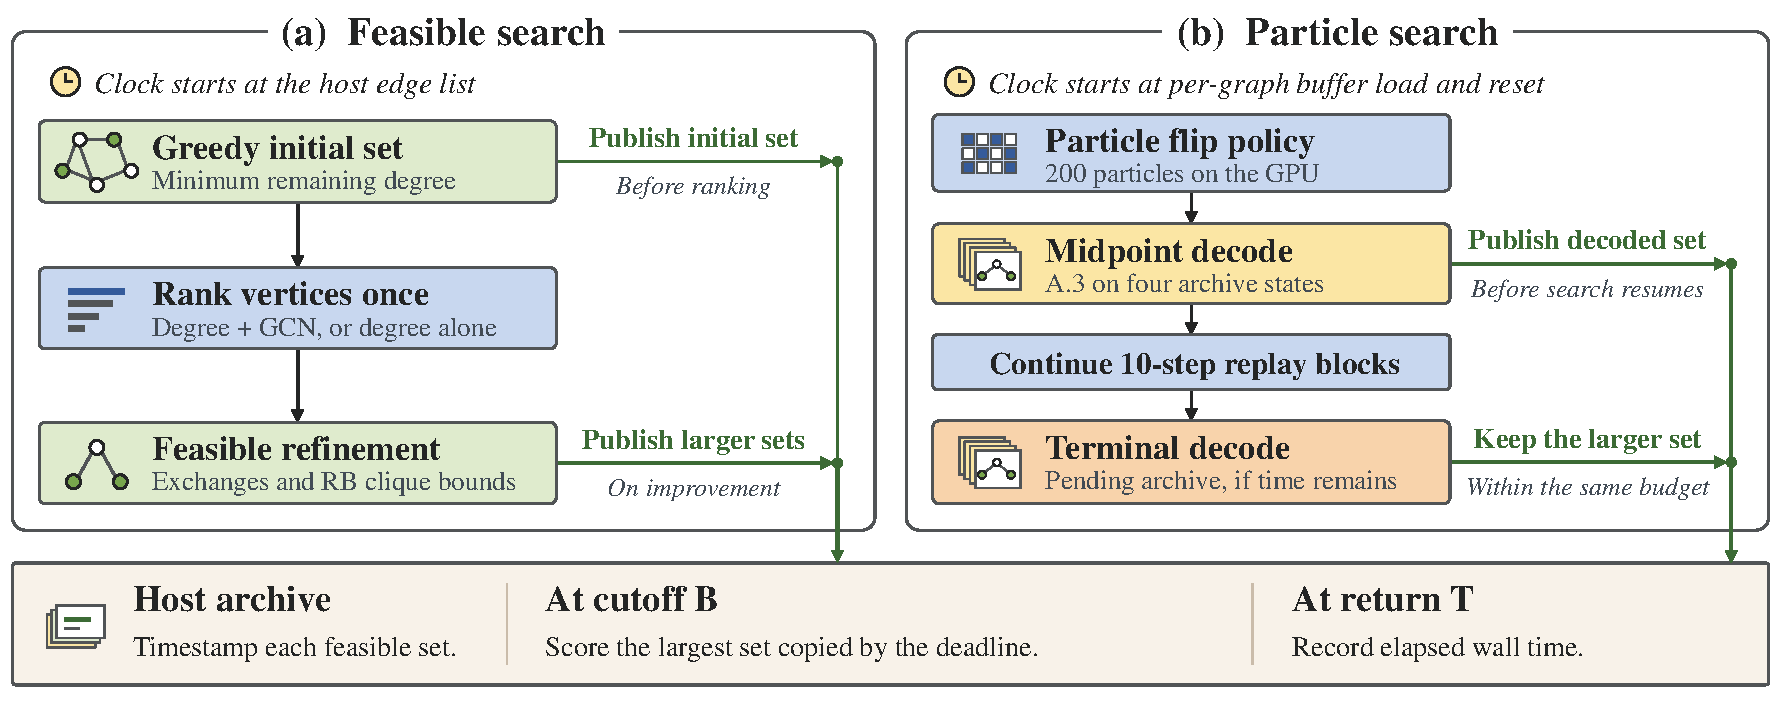
\includegraphics[width=.95\textwidth]{figures/search_paths.pdf}
\caption{\textbf{Two routes to an independent set before the deadline.} Panel titles name the routes: feasible search is SPRINT-C and particle search is SPRINT-S.
Dark arrows show execution order. Green arrows carry feasible vertex sets to the host.
(a) SPRINT-C publishes the greedy set before ranking vertices. The learned and degree-only rankings share the same refinement schedule.
(b) SPRINT-S publishes at the midpoint and again before return. Each readout decodes the four lowest-energy archive entries. Both decodes and their host copies count toward the per-graph budget.
At cutoff \(B\), the host scores the largest set it has received. The solver's return time \(T\) is recorded separately.}
\label{fig:search-paths}
\end{figure*}


For a graph \(G=(V,E)\), we seek the largest \(S\subseteq V\) with no edge inside \(S\). Figure~\ref{fig:search-paths} shows the two routes. SPRINT-C constructs an incumbent before running the network and then improves it. SPRINT-S explores conflicting states and pays a decode whenever it publishes an incumbent. In both designs the clock starts with the input in the representation the solver works from, and every published set is copied to a host archive with a timestamp.

\subsection{What can the host use at the cutoff?}
Let \(\tau_j\) be the elapsed time at which the vertices of a feasible set \(S_j\) have been copied to the host archive. At a deadline \(B\) we record
\begin{align}
 Q_B &= \max\bigl(\{\,|S_j|:\tau_j\leq B\,\}\cup\{0\}\bigr), \label{eq:score}\\
 C_B &= \mathbf{1}\{\,\exists j:\tau_j\le B\,\}. \label{eq:coverage}
\end{align}
A missed delivery contributes zero to the mean of \(Q_B\). On a covered run, \(t_B^*=\min\{\tau_j: |S_j|=Q_B,\ \tau_j\leq B\}\) is the earliest time the final score was readable. We also record the solve's return time \(T\): a set archived at 190~ms scores at a 200~ms cutoff even if the call returns at 205~ms. The three quantities separate what was delivered from what was computed. Comparisons pair runs on graph and search seed; for a contrast we average the per-graph differences and resample graphs (Appendix~\ref{app:protocol}). After timing, every archived set is verified against the input edges.

\subsection{The constructive route: publish before ranking}
\paragraph{Initialization and ranking.}
From the host edge list the solver builds a compressed sparse row adjacency, repeatedly adds a vertex of minimum remaining degree, and deletes its closed neighborhood, breaking ties with the search seed. When the residual graph is empty it publishes the resulting maximal independent set. The learned and degree-only arms share this initialization, so their first published set is identical and the first difference between them is the ranking.

Let \(d_v\) be the original degree and \(z_G(a)\) center and scale a vector across this graph's vertices, with a \(10^{-4}\) floor on the standard deviation. Refinement uses the priority
\begin{equation}
 p_v=z_G(-d)_v+\lambda\,z_G(g_\theta(G))_v .
 \label{eq:priority}
\end{equation}
The network \(g_\theta\) is a five-layer, width-128 graph convolutional encoder evaluated once on the GPU. A linear residual readout combines the final embedding with degree and neighborhood features. On each training graph we keep the four largest of eight OnlineMIS solutions and use a vertex's frequency across them as its soft membership target. One frozen checkpoint and \(\lambda=0.25\) serve every test set; the degree-only arm sets \(\lambda=0\) and skips the forward pass. Appendix~\ref{app:protocol} gives the training and validation criteria.

\paragraph{Feasible refinement.}
One CPU thread uses the priorities to exchange selected and unselected vertices. A one-for-two move replaces a selected vertex by two nonadjacent vertices for which it was the sole conflict. The archive keeps strict improvements. On RB instances the solver also branches over a partition into cliques: with partial solution \(P\) and \(k\) cliques still holding eligible vertices, every completion has size at most \(|P|+k\), and a branch closes when that bound cannot improve the incumbent. Small RB starts with branching, large RB starts with exchanges, and ER uses exchanges throughout; the register graphs use the frozen ER schedule. The clique phase publishes its best set on return.

\paragraph{Resident comparison.}
We run both rankings and native OnlineMIS afresh from the same host edge list at \(B\in\{50,100,200,500\}\)~ms on all four released test sets, with one CPU thread and a 3~ms return reserve. The clock includes graph conversion, search, host copies, and any GPU transfers and inference. OnlineMIS's greedy solution and subsequent best-solution updates reach the archive through an in-memory callback that copies vertices and timestamps each delivery, so the classical solver can also publish before its call returns. Library and weight loading precede each batch. Appendix~\ref{app:resident} gives branch allocations and the interleaved run order.

\subsection{The speculative route: particles and decode scheduling}
The speculative route uses the RLNN flip policy \citep{feng2025regularized}. It starts \(K=200\) binary particles from independent fair bits. At step \(t\) the policy maps the state \(x^k_t\) and the normalized adjacency with self-loops \(\widetilde A\) to vertex logits; with independent \(u^k_{v,t}\sim\mathrm{Unif}(0,1)\),
\begin{equation}
 x^k_{v,t+1}=x^k_{v,t}\ \oplus\
 \mathbf{1}\!\left\{u^k_{v,t}<\sigma(f_\theta(x^k_t,\widetilde A)_v)\right\},
 \label{eq:policy-step}
\end{equation}
where \(\oplus\) flips a bit when the indicator is one. Simultaneous flips can create conflicts. Each particle keeps its lowest-energy state; with \(c(x)=\sum_{\{u,v\}\in E}x_ux_v\) counting conflicting edges and \(s(x)=\sum_v x_v\), the archive ranks states by \(2\beta c(x)-s(x)\), which is \(\beta\) times the quadratic form of the symmetric unit-weight adjacency minus the cardinality. At a readout we decode the four lowest-energy archive entries with the released A.3 single-bit decoder, whose half-weight adjacency gives
\begin{equation}
 E_{\rm dec}(x)=\beta c(x)-s(x),\qquad \beta=1.02 .
 \label{eq:decode-energy}
\end{equation}
Removing a selected vertex with \(m\geq1\) selected neighbors changes \(E_{\rm dec}\) by \(1-\beta m<0\), and adding a conflict-free vertex lowers it by one. A one-flip local minimum is therefore a maximal independent set in exact arithmetic, which is what the decoder returns. We publish the largest decoded set.

\paragraph{Budgeting both readouts.}
The particle engine compiles the dense FP16 policy and replays ten-step CUDA Graph blocks with sparse archive-energy updates \citep{gray2019cudagraphs,ansel2024pytorch}. Its instance clock starts before filling reusable device buffers and resetting particles. Let \(\widehat h\) be the last synchronized block duration, and let \(r=\max(5\,\mathrm{ms},2\widehat d)\) be a decode reserve estimated from the latest decode time \(\widehat d\), taken from warm-up for the first graph. At elapsed time \(t\) we launch another block only when
\begin{equation}
 t+\widehat h+r<B .
 \label{eq:launch}
\end{equation}
The first block boundary at or after half the wall-clock budget triggers a readout, after which we raise \(r\) from the observed decode. A terminal readout decodes any pending archive if time remains; a late terminal copy leaves a timely midpoint incumbent in place. Comparing this schedule with terminal-only decoding isolates what publishing early is worth; fixed-work against fixed-deadline runs separate block cost from the extra search that faster blocks buy.

\section{Experiments}
\begin{figure}[t]
\centering
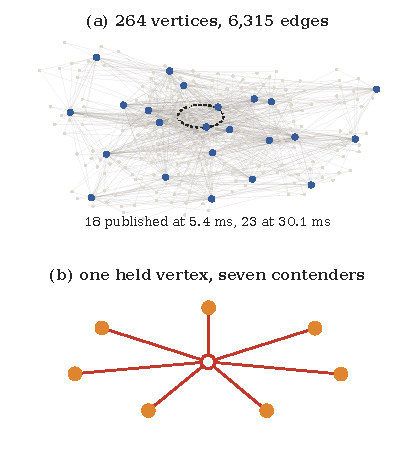
\includegraphics[width=.86\columnwidth]{figures/qualitative_instance.pdf}
\caption{\textbf{One instance, release to delivery.}
(a) Graph index~848 of RB-[200,300] (264 vertices, 6,315 edges). SPRINT-C publishes 18 vertices at 5.4~ms and delivers 23 at 30.1~ms (blue); the dashed circle marks the pocket in (b).
(b) The held vertex~149 conflicts with seven vertices that the final set selects, so none of the seven can join while it is held; exchanges drop such a vertex and admit its contenders. Resident OnlineMIS delivers 22 vertices on this graph at 7.8~ms.}
\label{fig:qualitative-instance}
\end{figure}


\label{sec:experiments}

\paragraph{Instances and protocol.}
The released MIS benchmarks contain 1,000 graphs each in RB-[200--300] and RB-[800--1200], 128 in ER-[700--800], and 16 in ER-[9000--11000] \citep{feng2025regularized}. Solvers are paired on graph ID and search seed (1017, 1019, 1021), giving 6,432 graph--seed pairs per budget, and at each of four budgets every resident solver runs on all pairs from the same host edge list. Table~\ref{tab:external-deadline} collects every measured method at the common 200~ms cutoff. The transfer study uses all 14 register interference graphs in the DIMACS COLOR catalog \citep{johnson1996dimacs}. We report mean delivered size with missed deliveries scored zero, the number of runs with a set on the host, and the actual return time. Paired contrasts average the three differences on each graph and resample graphs 5,000 times; all intervals are pointwise 95\%. Appendix~\ref{app:protocol} specifies training, validation and timing for every implementation.

\subsection{SPRINT-C delivers the largest set at 200 ms}
\begin{table*}[t]
\centering\footnotesize\setlength{\tabcolsep}{2.6pt}
\caption{Maximum independent set at 200\,ms per graph. Size averages the largest feasible set delivered to the host by the cutoff over all $N$ graph--seed pairs. A missed delivery scores zero. Ready counts timely deliveries. Time is the mean wall time per call in milliseconds, including overruns. DiffUCO skips inference on large RB and large ER after calibration. An em dash marks an unavailable measurement (Gurobi license details in Appendix~\ref{app:protocol}). Bold marks the highest mean size in each range.}
\label{tab:external-deadline}
\resizebox{\textwidth}{!}{\begin{tabular}{lrrrrrrrrrrrr}
\toprule
\paperHeader & \multicolumn{3}{c}{\paperHead{RB-[200--300]}} & \multicolumn{3}{c}{\paperHead{RB-[800--1200]}} & \multicolumn{3}{c}{\paperHead{ER-[700--800]}} & \multicolumn{3}{c}{\paperHead{ER-[9000--11000]}} \\
\paperHeader & \multicolumn{3}{c}{$N=3000$} & \multicolumn{3}{c}{$N=3000$} & \multicolumn{3}{c}{$N=384$} & \multicolumn{3}{c}{$N=48$} \\
\cmidrule(lr){2-4}\cmidrule(lr){5-7}\cmidrule(lr){8-10}\cmidrule(lr){11-13}
\paperHeader \paperHead{Solver} & \paperHead{Size\,$\uparrow$} & \paperHead{Time\,$\downarrow$} & \paperHead{Ready} & \paperHead{Size\,$\uparrow$} & \paperHead{Time\,$\downarrow$} & \paperHead{Ready} & \paperHead{Size\,$\uparrow$} & \paperHead{Time\,$\downarrow$} & \paperHead{Ready} & \paperHead{Size\,$\uparrow$} & \paperHead{Time\,$\downarrow$} & \paperHead{Ready} \\
\midrule
Gurobi (vertex MIP) & 16.5967 & 200.61 & 3000 & 32.0680 & 208.14 & 3000 & 29.8984 & 213.29 & 384 & \multicolumn{3}{c}{\textemdash} \\
KaMIS (ReduMIS CLI) & 1.8473 & 195.64 & 280 & 0.3490 & 202.75 & 26 & 0.0000 & 202.90 & 0 & 0.0000 & 206.18 & 0 \\
OnlineMIS (tuned CLI) & 20.0087 & 188.56 & 2994 & 41.6140 & 152.35 & 2997 & 42.5365 & 151.19 & 384 & 0.0000 & 206.15 & 0 \\
\rowcolor{TableOrange}
OnlineMIS (resident) & 20.0817 & 197.11 & 3000 & 41.7613 & 197.72 & 3000 & 42.7240 & 198.00 & 384 & 363.5833 & 197.48 & 48 \\
Released RLNN & 19.4247 & 152.25 & 2999 & 34.7923 & 166.72 & 2993 & 40.5469 & 145.57 & 383 & 0.0000 & 1606.14 & 0 \\
FLD-EG (recon.) & 18.3327 & 183.45 & 2999 & 35.3673 & 182.26 & 2999 & 34.9688 & 179.93 & 383 & 0.0000 & 346.88 & 0 \\
DiffUCO & 19.6473 & 52.22 & 3000 & 0.0000 & $<0.01$ & 0 & 42.8333 & 157.20 & 384 & 0.0000 & $<0.01$ & 0 \\
LTFT & 14.1917 & 191.25 & 3000 & 20.9747 & 195.55 & 3000 & 21.1562 & 198.41 & 383 & 3.7083 & 181.07 & 48 \\
DIFUSCO & 15.3523 & 161.78 & 2997 & 31.7993 & 94.99 & 3000 & 28.7109 & 165.92 & 355 & 0.0000 & 669.41 & 0 \\
DGL-TreeSearch & 5.0850 & 169.55 & 3000 & 6.1747 & 173.49 & 3000 & 9.4531 & 164.76 & 384 & 0.0000 & 25.30 & 0 \\
DIMES (ER retrain) & 18.9183 & 197.54 & 3000 & 35.4367 & 191.76 & 3000 & 37.4297 & 193.35 & 384 & 178.8542 & 279.00 & 30 \\
INTEL & 17.1893 & 200.24 & 3000 & 24.1410 & 200.23 & 3000 & 37.3620 & 201.16 & 384 & 65.6042 & 200.53 & 48 \\
PPO-LwD & 16.0697 & 190.43 & 3000 & 29.5217 & 192.71 & 3000 & 32.1667 & 193.29 & 384 & 208.1875 & 193.09 & 48 \\
DISCS iSCO & 19.3037 & 198.48 & 2960 & 0.1477 & 190.91 & 14 & 40.5677 & 196.05 & 383 & 0.0000 & 183.63 & 0 \\
RLSA & 19.9507 & 156.52 & 2999 & 31.2113 & 166.55 & 2527 & 43.1536 & 167.75 & 383 & 0.0000 & 2011.52 & 0 \\
iSCO (300 steps) & 11.4743 & 104.06 & 1804 & 0.1473 & 190.97 & 14 & 40.6146 & 195.74 & 383 & 0.0000 & 182.09 & 0 \\
\midrule
\rowcolor{TableGreen}
SPRINT-C (degree) & \textbf{20.1150} & 2.53 & 3000 & \textbf{42.4663} & 137.18 & 3000 & 44.2578 & 197.06 & 384 & 369.4167 & 197.27 & 48 \\
\rowcolor{TableBlue}
\textbf{SPRINT-C (learned)} & \textbf{20.1150} & 10.37 & 3000 & 42.4417 & 139.04 & 3000 & \textbf{44.3438} & 197.08 & 384 & \textbf{370.1250} & 197.24 & 48 \\
\bottomrule
\end{tabular}}
\end{table*}

At 200~ms SPRINT-C delivers the largest mean set of every measured solver on all four families (Table~\ref{tab:external-deadline}): 20.1150 against 20.0817 for resident OnlineMIS on small RB ($+0.0333$, $[0.0253,0.0420]$), 42.4417 against 41.7613 on large RB ($+0.6803$, $[0.6460,0.7153]$), 44.3438 against 42.7240 on small ER ($+1.6198$, $[1.5104,1.7292]$), and 370.1250 against 363.5833 on large ER ($+6.5417$, $[5.2917,8.0417]$). All 6,432 pairs receive a set, and on large RB the larger sets arrive sooner: 139.04 against 197.72~ms of mean return time. The same frozen configuration also beats RLSA on small ER by 1.1901 vertices ($[0.9635,1.5339]$) and the strongest neural baseline (INTEL, 17.1893) by 2.93 vertices on small RB.

Delivery itself separates the field. On small RB, where Gurobi's exact solver averages 16.5967, ReduMIS publishes a set on 280 of 3,000 pairs and DGL-TreeSearch on all 3,000 at 5.0850 vertices; on large ER, DIMES reaches 30 of 48 pairs and Gurobi's licence admits no model at that scale (Appendix~\ref{app:scale-supplement}). A score that mixes missed deadlines with delivered size ranks SPRINT-C first on every family, and the gap to each baseline is largest where coverage collapses.

\subsection{The win holds at every budget, and small RB is optimal}
\begin{figure*}[t]
\centering
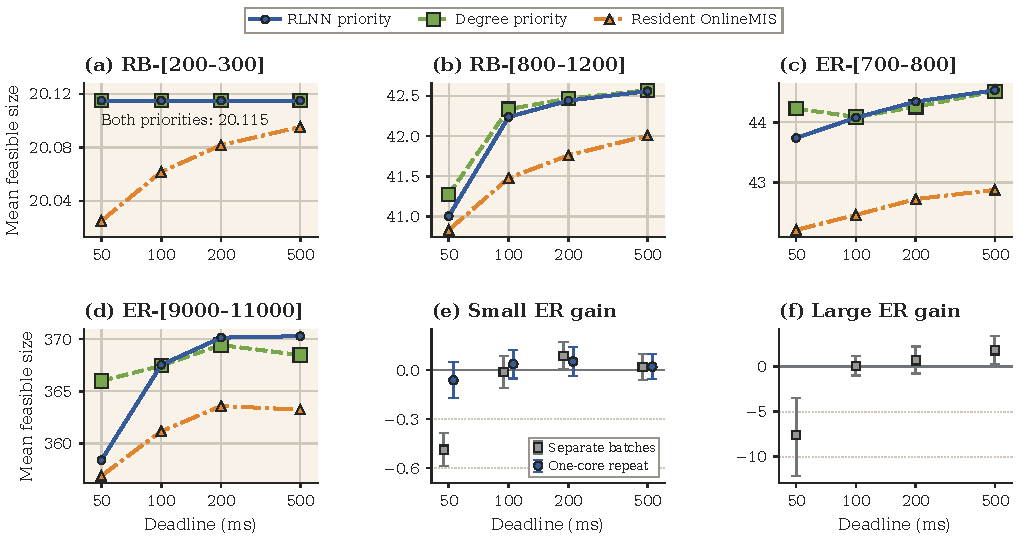
\includegraphics[width=.95\textwidth]{figures/resident_deadlines.pdf}
\caption{\textbf{Delivered size across four independently run deadlines.} (a--d) Mean feasible size at the cutoff over three seeds per graph. There are 1,000 graphs in each RB set, 128 in small ER and 16 in large ER. In (a), blue circles inside green squares mark identical optimal scores. (e--f) Mean size difference between learned and degree ranking on the two ER sets, with pointwise 95\% graph-bootstrap intervals. Panel (e) also shows a repeat interleaving all methods and budgets on one CPU core. Panel legend labels: ``RLNN priority'' is the learned ranking of SPRINT-C and ``Degree priority'' its degree ranking. Table~\ref{tab:resident-details} reports timing and delivery counts.}
\label{fig:resident-curves}
\end{figure*}

SPRINT-C leads resident OnlineMIS in each of the 16 family--budget combinations (Figure~\ref{fig:resident-curves}); the 50~ms large ER difference ($+1.50$, $[-3.19,6.04]$) is the only paired interval that includes zero. On RB-[200--300] SPRINT-C reaches all 3,000 offline-verified optima at every budget with one checkpoint: 375 graphs by a disjoint clique cover and the remaining 625 by an independent SAT check that no larger set exists (Appendix~\ref{app:protocol}). Both rankings attain those optima within 50~ms, at 2.53~ms average return for the degree arm and 10.37~ms for the learned arm; resident OnlineMIS climbs from 2,735 optimal sets at 50~ms to 2,941 at 500~ms. On the 14 register interference graphs the same checkpoint is optimal on all 42 pairs, and the shared greedy initializer reaches the optimum before either ranking is computed (Appendix~\ref{app:gain-sources}).

Figure~\ref{fig:qualitative-instance} follows one instance from release to delivery. The set published before inference already holds 18 vertices; exchanges then trade a held vertex for the candidates it blocks, and the run finishes at 23, one above resident OnlineMIS on the same graph.

Large RB shows why the archive, not the return value, is the quantity a caller can use. At 50~ms all 3,000 runs have a set on the host, yet only 2,525 calls finish before the deadline; at 200~ms resident OnlineMIS also delivers on large RB and small ER, with 190 and 41 calls still running when the budget expires (Table~\ref{tab:resident-details}). Appendix~\ref{app:gain-sources} separates how much of the delivered size comes from constructing and publishing a feasible set and how much from the learned ranking.

\subsection{Execution buys search depth}
On small RB SPRINT-S averages 20.0300 vertices in 193.80~ms, with paired gains of 0.6053 over released RLNN ($[0.5730,0.6387]$) and 0.0793 over RLSA ($[0.0613,0.1003]$) at the 200~ms cutoff (per-pair breakdown in Appendix~\ref{app:representation}, Figure~\ref{fig:baseline-pairs}). Holding the policy fixed, the execution protocol moves the operating point (Table~\ref{tab:policy-path}): with the released weights and 20 particles, fused inference gains 0.5527 vertices over released inference ($[0.5227,0.5847]$); raising the population to 200 adds 0.0587 ($[0.0467,0.0710]$) at the same weights; and the local checkpoint differs from the released one by $-0.0060$ ($[-0.0150,0.0033]$). Execution, not policy training, supplies the gain.

\begin{table}[t]
\caption{Inference protocol, particle count \(K\), and policy weights on the same 3,000 pairs at 200~ms. Steps count parallel updates per trajectory.}
\label{tab:policy-path}
\centering\small
\setlength{\tabcolsep}{3pt}
\begin{tabular}{@{}llrrrr@{}}
\toprule
\paperHeader
\paperHead{Protocol} & \paperHead{Weights} & \paperHead{\(K\)} & \paperHead{Size\,\(\uparrow\)} & \paperHead{Steps} & \paperHead{ms\,\(\downarrow\)} \\
\midrule
Released & Released & 20 & 19.4247 & 85.7 & 152.25 \\
SPRINT-S & Released & 20 & 19.9773 & 1357.9 & 195.84 \\
SPRINT-S & Released & 200 & 20.0360 & 346.2 & 193.87 \\
SPRINT-S & Local & 200 & 20.0300 & 351.0 & 193.80 \\
\bottomrule
\end{tabular}
\end{table}

At 130 steps, replay preserves decoded size at either compilation setting while cutting mean wall time from 277.70 to 74.53~ms (Table~\ref{tab:execution-ablation}). Under a 200~ms deadline the same switches raise search depth from 82.9 to 348.6 steps and add 0.3320 vertices ($[0.3093,0.3563]$); replay supplies 140.0 of the extra steps and compilation another 125.7. Because the fixed-work size is unchanged, the gain is more updates at the same per-step quality, not better updates. Dense adjacency and FP16 follow the same mechanism and add 0.1663 and 0.0493 vertices at fixed time (Appendix~\ref{app:representation}, Figure~\ref{fig:execution-effects}).


\begin{table}[t]
\caption{CUDA Graph replay and policy compilation on matched graph--seed pairs. Entries are means over 3,000 solves per configuration in each protocol.}
\label{tab:execution-ablation}
\centering
\small
\setlength{\tabcolsep}{3pt}
\begin{tabular}{llrrrrr}
\toprule
\paperHeader
 & & \multicolumn{2}{c}{\paperHead{130 steps}} & \multicolumn{3}{c}{\paperHead{200 ms}} \\
\cmidrule(lr){3-4}\cmidrule(lr){5-7}
\paperHeader
\paperHead{Replay} & \paperHead{Compile} & \paperHead{Size\,\(\uparrow\)} & \paperHead{ms\,\(\downarrow\)} & \paperHead{Size\,\(\uparrow\)} & \paperHead{Steps} & \paperHead{ms\,\(\downarrow\)} \\
\midrule
Off & Off & 19.8980 & 277.70 & 19.6967 & 82.9 & 184.07 \\
Off & On  & 19.8930 & 276.31 & 19.6907 & 79.6 & 183.91 \\
On  & Off & 19.8980 & 113.52 & 19.9890 & 222.8 & 192.22 \\
\rowcolor{TableGold}
On  & On  & 19.8930 & \textbf{74.53} & \textbf{20.0287} & \textbf{348.6} & 193.57 \\
\bottomrule
\end{tabular}
\end{table}

\subsection{Delivering earlier at equal size}
At 200~ms, midpoint-plus-terminal and terminal-only decoding both average 20.0303 vertices with full coverage, and their paired size difference is 0.0000 ($[-0.0017,0.0017]$). What changes is when the score exists: midpoint decoding moves the median time to the ultimately scored size from 194.24 to 106.63~ms, and by 125~ms it has published that size on 2,786 of 3,000 pairs, including 2,540 verified optima, where terminal-only decoding has published none. Depths are 351.81 and 353.62 steps and return times 193.55 and 194.03~ms, so the early readout buys availability without paying in quality (Figure~\ref{fig:intro-evidence}(a)). Decoding immediately after initialization costs 0.0187 vertices; Appendix~\ref{app:decode} follows one graph's membership and reports the leading, width and reserve variants.

\section{Discussion}

The two routes optimize different variables. SPRINT-S spends its budget on proposals and pays a decode whenever it needs a usable answer; it executed 4.2 times as many updates, and the extra proposals became larger sets. Early readout leaves size unchanged because by the midpoint most runs already hold a state that decodes to their eventual score, yet it changes when the caller can use that score. SPRINT-C instead holds a usable set from the first millisecond and only replaces an incumbent with a better one, which is why it reaches 11,000-vertex graphs whose padded buffers the particle pipeline cannot fill in time.

The lesson that should travel is that at a deadline the dominant decision is whether a feasible set is constructed and published before inference, not which order refines it. This is uncomfortable for a literature that optimizes the refinement step, and it is measurable only because the protocol timestamps every publication. Appendix~\ref{app:gain-sources} separates the two contributions and Appendix~\ref{app:rank-mix} shows the same ceiling under a weight sweep; learned ordering remains a genuine lever on the ER families and on no others.

\paragraph{Deployment reading.}
Rolling dispatch of perishable goods gives one instance: assignments name a shipment, a vehicle and a loading-to-delivery interval, and they conflict when they duplicate a shipment or overlap on a vehicle, so a maximal independent set is a feasible plan (Figure~\ref{fig:dispatch}, Appendix~\ref{app:dispatch}). The operational quantity is time to a feasible plan, which our protocol timestamps; accepted shipments and freshness violations would need field data \citep{zhang2020coldchain,stellingwerf2021quality}.

\paragraph{Scope.}
Our evidence covers four released synthetic families, 14 register interference graphs and four budgets, with schedules and the checkpoint fixed on independent validation graphs and timing conditional on one warmed server. Optimality is certified on RB-[200--300] and the register graphs; on the larger families we measure feasible cardinality. Unequal-value assignments need weighted independent set, and shared capacities of three or more assignments need extra constraints.


\section*{Impact Statement}
Short-budget selection can support time-sensitive planning. In a dispatch application the conflict graph, together with the temperature and capacity checks, determines which plans are operationally feasible. Our benchmark measures graph feasibility and computation time. Evaluating safety, product quality and service outcomes requires data and validation from the intended operation.

\section*{AI Disclosure Statement}
Generative AI tools assisted with literature search, experimental design and execution, analysis code, mathematical exposition, figures, and manuscript drafting. The numerical comparisons are based on solver outputs and per-instance timing records.

\urlstyle{same}
\bibliographystyle{icml2027}
\bibliography{references}

\clearpage
\appendix
\section{Solver configurations and statistical details}
\label{app:protocol}

\paragraph{Training and selection for SPRINT-C.}
We generate 128 training and 16 validation graphs for each of the two RB size ranges and the smaller ER range, separately from the released test graphs. On each training graph, eight OnlineMIS seeds supply independent sets. The target for a vertex is its frequency among the four largest sets. Starting from a locally trained RLNN encoder, we fine-tune the encoder and readout with class-balanced binary cross-entropy on these soft targets. AdamW uses learning rates $8{\times}10^{-5}$ for the encoder and $1.5{\times}10^{-3}$ for the readout. Of 24 epochs, epoch one maximizes the validation gain of greedily constructing a set in the predicted order relative to degree order, normalized by teacher size. The learned ranking uses this checkpoint throughout.

The 200~ms schedule reserves 3~ms for return. Small RB allocates up to 185~ms first to clique search and returns once optimality is established, using residual time for exchange otherwise. Large RB runs exchange first and reserves 175~ms for clique-based refinement, which can also solve smaller residual neighborhoods when the clique bound is loose. Small ER uses exchanges throughout. Both ranking variants share these validation-selected schedules. Large ER inherits the small ER schedule and checkpoint without additional tuning. Post hoc, a disjoint clique cover certifies the small RB optimum directly on 375 of 1,000 distinct graphs. On the other 625, an independent SAT check rules out an independent set larger than the delivered witness. In the initial 200~ms experiment, the learned solver also closed the bound within the timed call on 2,981 of 3,000 runs.

\paragraph{Frozen policy and hardware.}
The SPRINT-S checkpoint comes from a three-epoch local RLNN run initialized from a locally trained RB checkpoint, with 1,000 training graphs and 100 validation graphs. The network has five graph convolutional layers with 128 hidden units. Its default configuration uses 200 particles, a unit policy temperature, blocks of ten steps, and no initial decode. Each GPU configuration runs on a single RTX~5090 on the same Intel Xeon Platinum 8455C server. In the scale study, different configurations can use different RTX~5090 cards. Each card runs at most one of our timed jobs at once and shares the server with other workloads. The fused implementation uses PyTorch~2.9.1 with CUDA~13.0. SPRINT-S and its ablations are evaluated in separate batches. Small differences between repeats of the same configuration reflect separate wall-clock runs.

\paragraph{Paired estimand.}
For a method \(a\), let \(Q_{igs}^{a}\) denote the delivered size for graph \(g\), seed \(s\) and protocol \(i\). For two methods, the reported contrast for that protocol is
\begin{equation}
 \widehat{\Delta}_{a,b}=\frac{1}{n}\sum_{g=1}^n
       \frac{1}{|\mathcal S|}\sum_{s\in\mathcal S}
               (Q_{igs}^{a}-Q_{igs}^{b}).
\end{equation}
We resample the \(n\) graph means within each test set with replacement 5,000 times and report percentile intervals. Runs on the same graph stay together. For a fixed-step reference with a single observation per graph we reuse that observation within the graph. Intervals are pointwise for each comparison.

\subsection{External solver protocols}
The clock starts with the input in the representation expected by each solver. For example, LTFT receives a device-resident DGL graph and creates its rollout batch on the clock. INTEL receives a prepared adjacency matrix and constructs its graph convolution operator on the clock. SPRINT-S fills its reusable padded buffers on the clock. Priority-guided SPRINT-C starts from a host edge list and includes graph conversion, device transfers, scoring and feasible search in its time. Thus the times in Table~\ref{tab:external-deadline} measure solving from prepared input, including each implementation's per-solve work.

The method descriptions apply across the four columns of Table~\ref{tab:external-deadline}. The paired comparisons below use SPRINT-S on RB-[200--300]. For transfer, the particle methods retain their weights, particle counts and stopping rules. DIFUSCO selects its denoising step count separately on each split using a 180~ms calibration target on the graph with the most edges. DiffUCO and DGL-TreeSearch can skip the first search block when its estimated duration exceeds the budget. A zero score can therefore accompany a short return time. Conversely, an uninterruptible operation can return after the deadline.
DISCS iSCO uses the official MIS model and path auxiliary sampler \citep{sun2023revisiting,goshvadi2023discs}. Its full-window variant continues the 300-step cooling schedule until the deadline. RLSA retains its small-graph settings and uses midpoint and terminal A.3 decoding. KaMIS OnlineMIS \citep{dahlum2016accelerating} and ReduMIS \citep{lamm2017finding} each use one CPU thread. For the executable-based runs the 200~ms clock includes starting the process, reading its prepared input and collecting its solution on exit. For the tuned OnlineMIS row in Table~\ref{tab:external-deadline}, we run internal limits of 120, 150 and 180~ms on 16 independent validation graphs per regime (seed 517). We choose the largest mean delivered size, breaking ties in favor of the longer limit. Validation selects 180~ms on small RB and large ER, and 120~ms on large RB and small ER. All three limits score zero on the independent large ER validation graphs. The selected CLI then times out on all 48 large ER test pairs. Table~\ref{tab:scale-supplement} uses a fixed 180~ms limit for both executables. We verify all scored sets against the original edges.

\paragraph{Released RLNN and reconstructed FLD-EG.}
Under the 200~ms deadline, released RLNN uses the authors' RB-small ERDOES checkpoint, 20 particles, and a 100-step cap. FLD-EG is our PyTorch reconstruction of Algorithm~1 and Table~3 of \citet{wang2025fractional}, with 200 particles and a 300-step cap. The deadline harness uses midpoint and terminal decoding for both methods, with A.3 decoding for released RLNN and per-chain greedy decoding for FLD-EG. Both deliver 2,999 on-time solutions. The paired size gains of SPRINT-S are \(0.6053\) over released RLNN (95\% CI \([0.5730,0.6387]\)) and \(1.6973\) over the FLD-EG reconstruction (95\% CI \([1.6457,1.7487]\)). Both baselines return sooner on average than SPRINT-S (193.80~ms).

\paragraph{DiffUCO and LTFT.}
DiffUCO \citep{sanokowski2024diffusion} uses the RB-small checkpoint released with the SDDS comparison \citep{sanokowski2025sdds} and timed conditional-expectation decoding. It finishes 141.58~ms faster on average, while SPRINT-S returns larger sets by the shared deadline (paired gain \(0.3827\), 95\% CI \([0.3497,0.4163]\)). We retrain LTFT \citep{zhang2023flows} with its official code for 20 epochs on 4,000 independently generated RB-small graphs. At the deadline, 2,448 of its 3,000 scored sets can still be extended by at least one vertex. All runs of both baselines deliver a feasible set on time. The paired gain of SPRINT-S over LTFT is \(5.8383\) (95\% CI \([5.7143,5.9660]\)).

\paragraph{DIFUSCO and DGL-TreeSearch.}
We transfer the released DIFUSCO categorical MIS checkpoint \citep{sun2023difusco} from SATLIB to RB, using four cosine-scheduled denoising steps and the released greedy decoder. It delivers a set on time in 2,997 runs. We retrain DGL-TreeSearch \citep{boether2022tree} on 4,000 independent RB graphs labeled by OnlineMIS. Its single-worker search processes up to four probability maps per expansion and averages 2.77 expansions, with partial independent sets eligible for scoring. In 483 runs the search returns after 200~ms but has already delivered a feasible set. The paired size gains of SPRINT-S are \(4.6777\) over DIFUSCO (95\% CI \([4.5887,4.7670]\)) and \(14.9450\) over DGL-TreeSearch (\([14.8080,15.0810]\)).

\paragraph{INTEL and PPO-LwD.}
For INTEL \citep{li2018guided}, we use the released 20-layer GCN weights and check the 32 output probability maps of our FP32 GPU port against the released TensorFlow graph on a fixed input. A single worker samples from the search queue and retains independent prefixes, with the optional reduction and local search disabled. For PPO-LwD \citep{ahn2020defer}, we retrain the released policy for 250 PPO updates over two passes through 4,000 independent RB graphs. We select the checkpoint on 64 held-out graphs, then score the largest accepted independent set across ten parallel trajectories after each action, up to 32 actions per trajectory.

Both methods deliver an independent set within 200~ms in all 3,000 runs. SPRINT-S gains \(2.8407\) vertices over INTEL (95\% CI \([2.7590,2.9243]\)) and \(3.9603\) over PPO-LwD (\([3.8697,4.0533]\)). It matches or exceeds both baselines on every graph--seed pair. INTEL and PPO-LwD return after the cutoff in 1,667 and 235 runs, respectively, for which we score the best set already available at 200~ms.

\subsection{Classical solvers and matched policies across scales}
\label{app:scale-supplement}
\begin{table*}[t]
\centering\footnotesize\setlength{\tabcolsep}{3.8pt}
\caption{Fixed-limit KaMIS executables and distribution-matched RLNN under the 200\,ms deadline. Both KaMIS executables use a 180\,ms internal limit on all four sets. Size averages the delivered cardinality across all $N$ graph--seed pairs, with missed deliveries scored zero. Time is mean wall time in milliseconds. Ready counts pairs with a feasible set by the cutoff. RLNN uses the released checkpoint for each RB range and the shared ER checkpoint for both ER ranges.}
\label{tab:scale-supplement}
\resizebox{\textwidth}{!}{\begin{tabular}{lrrrrrrrrrrrr}
\toprule
\paperHeader & \multicolumn{3}{c}{\paperHead{RB-[200--300]}} & \multicolumn{3}{c}{\paperHead{RB-[800--1200]}} & \multicolumn{3}{c}{\paperHead{ER-[700--800]}} & \multicolumn{3}{c}{\paperHead{ER-[9000--11000]}} \\
\paperHeader & \multicolumn{3}{c}{$N=3000$} & \multicolumn{3}{c}{$N=3000$} & \multicolumn{3}{c}{$N=384$} & \multicolumn{3}{c}{$N=48$} \\
\cmidrule(lr){2-4}\cmidrule(lr){5-7}\cmidrule(lr){8-10}\cmidrule(lr){11-13}
\paperHeader \paperHead{Solver} & \paperHead{Size\,$\uparrow$} & \paperHead{Time\,$\downarrow$} & \paperHead{Ready} & \paperHead{Size\,$\uparrow$} & \paperHead{Time\,$\downarrow$} & \paperHead{Ready} & \paperHead{Size\,$\uparrow$} & \paperHead{Time\,$\downarrow$} & \paperHead{Ready} & \paperHead{Size\,$\uparrow$} & \paperHead{Time\,$\downarrow$} & \paperHead{Ready} \\
\midrule
KaMIS OnlineMIS & 20.0393 & 186.86 & 2998 & 6.8280 & 200.99 & 503 & 11.6224 & 200.42 & 104 & 0.0000 & 206.12 & 0 \\
KaMIS ReduMIS & 1.8473 & 195.64 & 280 & 0.3490 & 202.75 & 26 & 0.0000 & 202.90 & 0 & 0.0000 & 206.18 & 0 \\
Released RLNN (matched) & 19.4247 & 152.25 & 2999 & 30.5393 & 173.85 & 2590 & 40.5521 & 177.93 & 383 & 0.0000 & 1552.01 & 0 \\
\bottomrule
\end{tabular}}
\end{table*}

Table~\ref{tab:scale-supplement} reports the fixed-limit executable runs. On larger RB graphs, OnlineMIS delivers on 503 of 3,000 pairs with a 180~ms internal limit, versus 2,997 with the validation-selected 120~ms limit. The corresponding mean delivered sizes are 6.8280 and 41.6140. For released RLNN, the matched-weight row uses the public RB-large checkpoint on larger RB graphs and the public ER checkpoint on both ER sets, with the original 20-particle, 100-step cap. On small ER graphs, its mean size is 40.5521, compared with 40.5469 using RB-small weights.

On large RB, full-window iSCO delivers on 14 of 3,000 runs. The 14 timely sets average 31.6429 vertices, yielding 0.1477 across all runs. On large ER, LTFT delivers on all 48 runs. Each action can add at most one vertex per trajectory. With three to five actions per run, the delivered sets contain three to five vertices and average 3.7083.

\paragraph{DIMES.} We train the released MIS meta-solver \citep{qiu2022dimes} on 128 independently generated ER-[700--800] training graphs. The local configuration uses one heatmap, 32 sampled trajectories, one inner meta-update and minibatches of eight graphs. We fix the fourth-epoch checkpoint (64 outer updates) before evaluation and transfer it unchanged to all four test sets. Inference starts from the host edge list and charges sparse graph construction, the FP32 network forward pass, transfers and decoding to the deadline. A greedy readout produces the first candidate. Further batches sample feasible sets from the heatmap. Each completed batch can publish its largest set. We timestamp copies of the actual vertices. We keep the parameters fixed at test time. On a 47-vertex reference graph the FP32 port agrees with the upstream TensorFlow scores to within $2.32\times 10^{-5}$ in maximum absolute error and yields the same greedy vertices.

\paragraph{Gurobi.} For Gurobi~\citep{gurobi2026}, introduce one binary variable $x_v$ for each vertex of degree $d_v$ and maximize $\sum_v x_v$ subject to
\[
 d_v x_v + \sum_{u\in N(v)} x_u \le d_v \qquad (v\in V).
\]
Selecting $v$ forces every neighbor to zero. The model uses one linear row per vertex and has the same feasible binary sets as the edge formulation. A single solver thread starts from the host edge list. The timer covers sparse matrix and model construction, optimization, copying incumbent vertices from solution callbacks, and model disposal. A solved instance may yield an incumbent before the call returns. The available Gurobi~13.0.3 license admits at most 2,000 variables and 2,000 linear rows. The first large ER model has 9,904 of each, so there is no large ER Gurobi timing or score.

\paragraph{The largest ER graphs.} The 16 graphs have 9,004--10,915 vertices and 809,362--1,190,799 undirected edges. We ran the three resident methods in separate batches, pinned to the same CPU core. The two priority arms start from identical vertex sets on each pair, averaging 341.9583 vertices. In the 200~ms run the learned solver publishes its initial set after a median of 18.31~ms. The median time to its final scored size is 130.90~ms. At 200~ms both priority arms return within the deadline on all 48 pairs, as does OnlineMIS on 46.

DiffUCO calibrated its two trajectories at 36.29 and 37.91 seconds using the JAX platform allocator. Its scheduler skipped both trajectories in all 48 timed solves and returned in under 0.01~ms on average. DIFUSCO attempted a trajectory on every run. Even its shortest calibrated trajectory (one denoising step followed by greedy decoding) took 785~ms on the calibration graph. It delivered no feasible set by 200~ms across the 48 runs, with a mean return time of 669.41~ms.

\subsection{OnlineMIS seed replication}
\label{app:seeds}
Table~\ref{tab:seeds} uses the same 1,000 test graphs throughout. The original cohort uses seeds 1017, 1019, 1021. The replication uses 1023, 1025, 1027. OnlineMIS is a randomized local-search algorithm. We retain all runs of both solvers, including misses. For the pooled interval, we average all six paired differences within each graph before resampling graphs.

In the primary cohort, OnlineMIS averages 186.86~ms and delivers 2,998 sets on time. SPRINT-S wins 126 pairs, ties 2,679 and loses 195. Across all six seeds, mean wall times are 187.08~ms for OnlineMIS and 193.79~ms for SPRINT-S. SPRINT-S delivers on all 6,000 pairs. OnlineMIS leads by 0.0264 vertices on the 5,995 pairs with two timely deliveries. In the separate three-seed ReduMIS run, mean wall time is 195.64~ms. Its 280 timely sets average 19.7929 vertices, yielding a mean score of 1.8473 over all 3,000 runs.

\begin{table}[t]
\centering\small\setlength{\tabcolsep}{3pt}
\caption{Seed replication at 200~ms. Size includes all runs. The interval compares SPRINT-S with OnlineMIS (SPRINT-S minus OnlineMIS).}
\label{tab:seeds}
\begin{tabular}{@{}lrrr@{}}
\toprule
\paperHeader
\paperHead{Seed panel} & \paperHead{SPRINT-S} & \paperHead{OnlineMIS} & \paperHead{Paired gain [95\% CI]} \\
\midrule
Original & 20.0300 & 20.0393 & $-.0093$ [$-.0330,.0177$]\\
Additional & 20.0247 & 20.0337 & $-.0090$ [$-.0357,.0203$]\\
\rowcolor{TableGold}
All six & 20.0273 & 20.0365 & $-.0092$ [$-.0300,.0122$]\\
\bottomrule
\end{tabular}
\end{table}

\subsection{Fixed-work reference points}
\label{app:fixed}
\begin{table}[t]
\caption{Observed quality and mean solver latency on RB-[200--300]. The reference methods use their fixed-step configurations.}
\label{tab:main}
\centering
\begin{tabular}{lrr}
\toprule
\paperHeader
\paperHead{Solver} & \paperHead{Mean size\,$\uparrow$} & \paperHead{Mean ms\,$\downarrow$} \\
\midrule
Released RLNN & 19.520 & 208.07 \\
Fixed-step RLSA & 19.973 & 208.39 \\
SPRINT-S with PAVE & 20.0147 & 185.75 \\
\midrule
\rowcolor{TableBlue}
\textbf{SPRINT-S} & \textbf{20.0300} & 193.80 \\
\bottomrule
\end{tabular}
\end{table}

\paragraph{Comparison with the released solvers.}
With PAVE disabled, SPRINT-S returned a feasible solution within 200~ms on all 3,000 graph--seed pairs in the primary cohort. Its paired mean size gain over released RLNN is \(0.510\) (95\% CI \([0.476,0.546]\)). The paired gain over the fixed-step RLSA reference is \(0.057\) (95\% CI \([0.040,0.074]\)). This comparison estimates the difference between the observed operating points in Table~\ref{tab:main}.


\subsection{Amortization and deployment boundary}
\begin{figure*}[t]
\centering
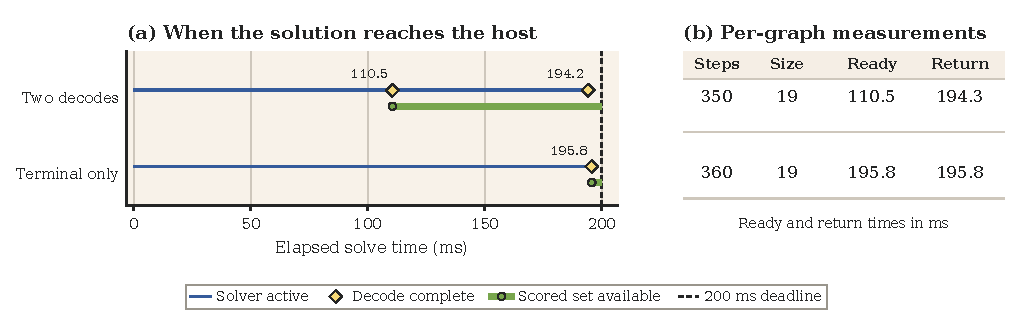
\includegraphics[width=\textwidth]{figures/solve_clock.pdf}
\caption{\textbf{Two decoding schedules on the same RB graph} (242 vertices, seed 1017). (a) Timing starts with per-graph buffer loading and particle reset. The blue line ends when the solver returns. Diamonds mark completed decodes. The green segment starts when the ultimately scored set reaches the host and extends to the 200~ms deadline. The midpoint decode yields 19 vertices at 110.5~ms, and the terminal decode at 194.2~ms ties that size. With only a terminal decode, 19 vertices become available at 195.8~ms. (b) The two runs reach the same size in 350 and 360 steps, respectively.}
\label{fig:solve-clock}
\end{figure*}

Figure~\ref{fig:solve-clock} follows the same graph and seed under two decode schedules. The mid-run copy makes the eventual 19-vertex set available 85.3~ms earlier, before the particle call returns.

Across the three 1,000-graph batches in the fixed-130-step experiment, mean recorded engine setup takes 0.79~s for uncompiled eager execution and 5.51~s for compiled replay. Adding measured setup to the full evaluation loop gives 283.45~s and 86.46~s per batch, respectively. The loop includes graph preparation and per-instance solves. Both totals start after loading the weights and scanning dataset shapes. These measurements describe repeated inference on graphs that fit the same buffers. Deployments with occasional single requests would also pay any unamortized loading, warm-up and compilation costs.


\subsection{SPRINT-S decoding and refinement}
\label{app:decode}
\begin{figure*}[t]
\centering
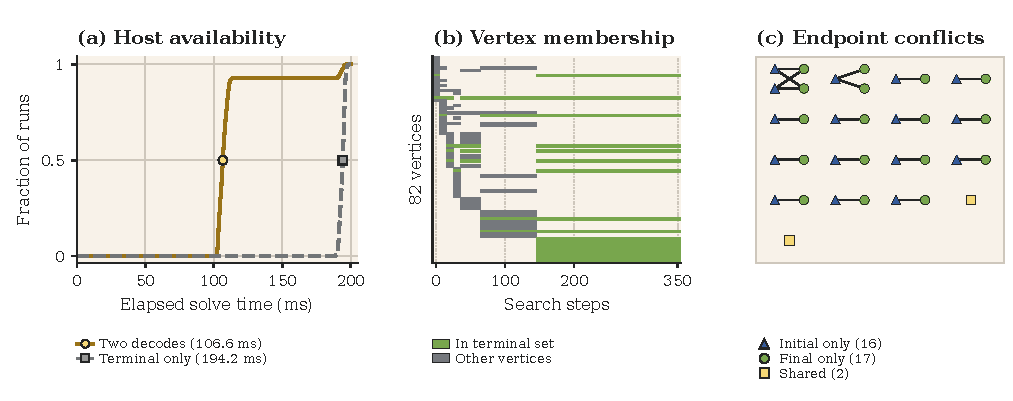
\includegraphics[width=\textwidth]{figures/decode_cases.pdf}
\caption{\textbf{Host availability and changing membership in SPRINT-S.} (a) Across 3,000 small RB graph--seed pairs, the median time at which the ultimately scored set reaches the host is 106.6~ms with two decodes and 194.2~ms with terminal-only decoding. Markers locate the medians on the cumulative curves. (b) A separate fixed-work run on the first RB graph (242 vertices, 2,393 edges, seed 1017) decodes the top four archive entries every ten steps. Each row tracks one vertex. Filled cells mark membership at that checkpoint, and green identifies vertices that belong to the terminal set. Size reaches 19 at step ten and stays there while membership changes. (c) The union of the initial and final sets induces 19 conflict edges. The two shared vertices are isolated.}
\label{fig:decode-cases}
\end{figure*}

\paragraph{An instance at constant cardinality.}
Figure~\ref{fig:decode-cases} follows the first test graph and the first search seed in a separate diagnostic. We decode the top four archived states at initialization and after every ten steps through step 350. The initial set has 18 vertices. By step ten it has 19, and the size then stays at 19 even as the membership changes. The initial and terminal sets share just two vertices. Their union contains 19 conflict edges, all between vertices exclusive to different sets. This illustrates why an archive can continue changing after its best decoded size has plateaued, and why splicing two feasible candidates would require checking conflicts again. The diagnostic uses step counts so that observing these intermediate states does not enter the latency experiment.

\paragraph{Decode width.}
In a separate paired run, increasing the decode width from the four lowest-energy states to all 200 particles raises mean decode time per solve from 2.12 to 4.67~ms. The mean search depth falls from 354.85 to 346.82 steps. The wider decode nevertheless increases size from 20.0300 to 20.0350 (\(+0.0050\), 95\% CI \([0.0013,0.0090]\)). Both widths have 3,000 on-time feasible incumbents. Returning from the solve takes more than 200~ms in 12 all-particle runs and zero four-particle runs. Only 27 of the 3,000 paired scores differ. Searching deeper and examining a wider archive can each improve the answer, but the width benefit here is concentrated in a small fraction of instances.

\paragraph{Using the remaining time.}
We compare three uses of the final 40~ms. Returning the search incumbent with the reserve unused gives mean size 20.0123 after 274.85 steps (153.54~ms). Using the reserve for a learned local postprocessor (PAVE) gives 20.0147 after 278.39 search steps (185.75~ms), a paired gain of 0.0023 (95\% CI \([-0.0003,0.0053]\)). PAVE improves its own incoming incumbent on 10 runs. Keeping the time for further neural search gives 20.0300 after 350.98 steps (193.80~ms), a gain of 0.0177 over the unused reserve (\([0.0123,0.0233]\)) and 0.0153 over PAVE (\([0.0097,0.0213]\)). All three configurations deliver a feasible set in all 3,000 runs. Nine PAVE runs return after the deadline and receive credit for the earlier incumbent. These contrasts use the same graph--seed pairs in separate batches.

\subsection{Variation within the released test split}
\label{app:strata}
We group all 1,000 graphs by their observed number of vertices and retain all three primary seeds per graph. Table~\ref{tab:strata} reports descriptive paired means. SPRINT-S gains vertices over both released RLNN and RLSA in each group. OnlineMIS has a small mean advantage in each. Differences across these groups combine size with any graph structure that varies with size in the RB generator.

\begin{table}[h]
\centering\small
\setlength{\tabcolsep}{3pt}
\caption{Mean size and paired size differences by graph order at 200~ms. The final three columns subtract the named comparator from SPRINT-S.}
\label{tab:strata}
\begin{tabular}{@{}lrrrrr@{}}
\toprule
\paperHeader
\paperHead{Nodes} & \paperHead{Graphs} & \paperHead{SPRINT-S} & \paperHead{RLNN} & \paperHead{RLSA} & \paperHead{OnlineMIS} \\
\midrule
200--219 & 340 & 19.8235 & +0.5010 & +0.0637 & $-$0.0049 \\
220--239 & 363 & 19.4077 & +0.5969 & +0.0707 & $-$0.0138 \\
240--264 & 297 & 21.0269 & +0.7351 & +0.1077 & $-$0.0090 \\
\bottomrule
\end{tabular}
\end{table}

\subsection{Weight of the learned ranking and rank agreement}
\label{app:rank-mix}
The learned arm of SPRINT-C in Table~\ref{tab:external-deadline} uses $\lambda=0.25$ in Eq.~\eqref{eq:priority}. We re-ran the same search with $\lambda\in\{0.1,1.0\}$ and with the learned score alone ($\lambda=\infty$, no degree term), from the same checkpoint and schedules as the shipped solver, and added a degree arm to the same batch so that batch drift cancels. Table~\ref{tab:rank-mix} reports delivered size. On RB-[200--300] every arm attains the same 20.1150 vertices. On RB-[800--1200] the learned term is worth 0.019 to 0.074 vertices over degree, and the gain grows with $\lambda$. On ER-[700--800] the shipped $\lambda=0.25$ is best (0.1745 over degree, $[0.0911,0.2552]$), $\lambda=0.1$ loses 0.107 and the learned score alone gains 0.133. On the 16 large ER graphs all arms lie within 1.25 vertices of degree and every interval includes zero.

The blend is nearly a monotone function of degree: the Spearman correlation between the blended priority and $-d$ is 0.990, 0.991 and 0.999 on small RB, large RB and small ER. The learned score alone is less redundant (0.583, 0.645 and 0.956), and its top 5\% overlaps the degree top 5\% by only 0.13, 0.18 and 0.72, so the sweep does test a different order; what that order buys in delivered size stays within the ranges above. The blend therefore reorders vertices whose degree ranks are already close, which bounds what a change of ranking can add to this search.

\begin{table}[h]
\centering\footnotesize
\setlength{\tabcolsep}{4pt}
\caption{Delivered size at 200~ms as the weight $\lambda$ of the learned term in Eq.~\eqref{eq:priority} varies, measured in one batch against a degree arm. RB small is RB-[200--300], RB large RB-[800--1200], ER small ER-[700--800], ER large ER-[9000--11000]. The last row drops the degree term; $\lambda=0.25$ is shipped.}
\label{tab:rank-mix}
\begin{tabular}{@{}lrrrr@{}}
\toprule
\paperHeader
\paperHead{Mix} & \paperHead{RB small} & \paperHead{RB large} & \paperHead{ER small} & \paperHead{ER large} \\
\midrule
Degree only & 20.1150 & 42.4387 & 44.2500 & 365.6250 \\
$\lambda=0.1$ & 20.1150 & 42.4573 & 44.1432 & 364.3958 \\
$\lambda=0.25$ & 20.1150 & 42.4933 & 44.4245 & 365.7083 \\
$\lambda=1$ & 20.1150 & 42.4950 & 44.2005 & 365.5833 \\
Learned only & 20.1150 & 42.5130 & 44.3828 & 364.3750 \\
\bottomrule
\end{tabular}
\end{table}

\subsection{Representation, precision, and the scale boundary}
\label{app:representation}
\begin{figure*}[!t]
\centering
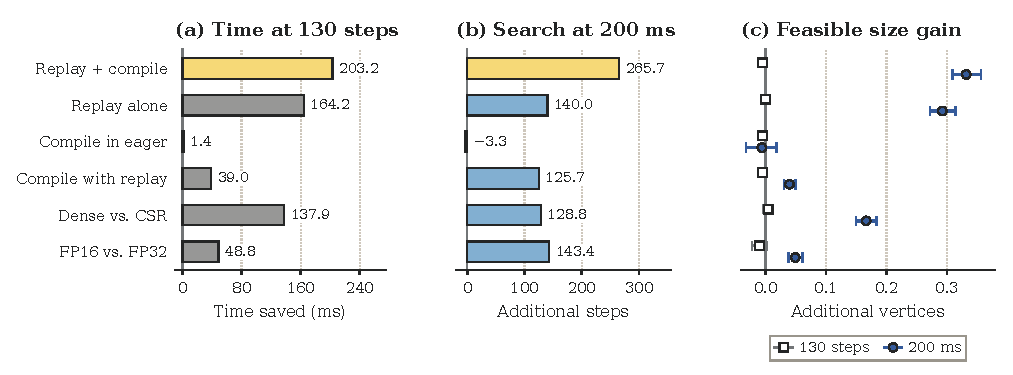
\includegraphics[width=.95\textwidth]{figures/execution_effects.pdf}
\caption{\textbf{How execution changes SPRINT-S.} Each row compares matched runs on 1,000 small RB graphs and three seeds. Gold bars mark the joint switch from eager, uncompiled execution to compiled CUDA Graph replay. The next three rows separate these switches. Both adjacency formats use uncompiled replay. The precision comparison uses compiled replay with TF32 disabled. (a) Time saved at 130 steps. (b) Additional steps within 200~ms. (c) Mean paired gain in delivered size under each protocol, with pointwise 95\% graph-bootstrap intervals.}
\label{fig:execution-effects}
\end{figure*}

\begin{figure*}[t]
\centering
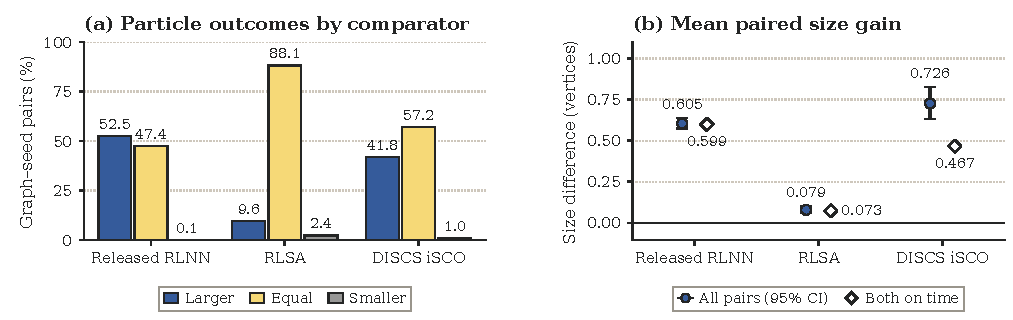
\includegraphics[width=.95\textwidth]{figures/baseline_pairs.pdf}
\caption{\textbf{SPRINT-S on small RB graphs at 200~ms.} (a) Percentage of 3,000 matched graph--seed pairs on which the particle solver delivers a larger, equal or smaller set than each comparator. (b) Blue circles give the mean paired size difference over all pairs, with misses scored zero. Whiskers show pointwise 95\% intervals from resampling the 1,000 graphs after averaging each graph's three seed differences. Open diamonds give the mean over pairs on which both solvers deliver on time.}
\label{fig:baseline-pairs}
\end{figure*}

Switching from CSR to dense adjacency with compilation off reduces 130-step time from 252.02 to 114.15~ms while the fixed-work size difference is 0.0047 ($[-0.0033,0.0127]$); at 200~ms dense search buys 128.84 more steps and 0.1663 vertices ($[0.1497,0.1833]$). With replay and compilation on, FP16 reduces 130-step time from 127.49 to 78.65~ms, and the size difference moves from $-0.0100$ ($[-0.0227,0.0023]$) at fixed work to $+0.0493$ ($[0.0383,0.0610]$) at fixed time. Precision changes both the policy and the sampled states, so part of that gain is accuracy lost in the search itself. All four arms publish on every pair.

The particle route was sized for small graphs and does not transfer upward unchanged. On RB-[800--1200] it averages 28.9847 vertices with 2,613 timely deliveries, below the 30.5393 of the released solver using its large-RB checkpoint; on ER-[9000--11000], filling one graph's padded buffers alone takes at least 1.84~s and all 48 runs miss the cutoff. The multi-scale results in Table~\ref{tab:external-deadline} therefore rest on feasible search, whose cost grows with the search rather than with the instance buffer.

\subsection{What the constructive gain is made of}
\label{app:gain-sources}
Both priority arms start from the same greedy set and use the same exchanges and branches, so their difference isolates the ranking. Degree ordering alone delivers 20.1150 and 42.4663 on the two RB families, 44.2578 on small ER and 369.4167 on large ER, so the learned scores differ by 0, $-0.025$, 0.086 and 0.708 vertices. On large ER the sign of that comparison depends on the budget: at 50~ms the learned arm loses 7.5833 vertices to degree ($[-12.1250,-3.4375]$), at 500~ms it gains 1.8125 ($[0.2708,3.3958]$). Learned guidance accounts for a family-dependent share and the construction and publication of a feasible set accounts for the rest.

On the 14 register graphs two adjacent vertices cannot share a register. With the original edges, the frozen checkpoint and the ER exchange schedule, all three resident solvers return on time and reach a mean of 208.3571; a matching clique-cover bound certifies every solution on all 42 graph--seed pairs. The shared greedy initializer is already optimal on every run, before either ranking is computed; OnlineMIS starts at 178.0476 and reaches the optimum after a median of 1.48~ms. These instances separate time-to-optimum from final size and show the ceiling of the ranking.

\section{Initial 200 ms feasible-search comparison}
\label{app:initial-priority}
The first evaluation of the frozen checkpoint compared learned and degree rankings with the validated OnlineMIS executable. Learned search averaged 20.1150, 42.4803 and 44.3620 vertices on small RB, large RB and small ER, with mean return times of 9.81, 136.64 and 197.07~ms. It delivered on all 6,384 runs. The paired gain was 0.8663 ($[0.8033,0.9547]$) over the tuned executable on large RB and 1.2083 ($[0.9818,1.5547]$) over RLSA on ER. On small RB, degree search matched every learned score and returned in 5.30~ms on average. On large RB and ER the learned-minus-degree differences were 0.0087 ($[-0.0063,0.0237]$) and 0.0807 ($[-0.0026,0.1641]$). On ER, setting every priority to zero gave a mean of 44.1927 and a learned-minus-flat difference of 0.1693 ($[0.0729,0.2578]$).

For the same three graph sets, Table~\ref{tab:external-deadline} reports a separate common-interface run for learned ranking, degree ranking and resident OnlineMIS on the original graph--seed pairs. The executable and resident OnlineMIS rows thus reflect two different ways of delivering the classical solver's set.

\section{Common-input deadline experiments}
\label{app:resident}
\begin{table*}[t]
\centering\scriptsize\setlength{\tabcolsep}{4.8pt}
\caption{Resident solvers at four independently run deadlines. Size averages the largest feasible set on the host by the cutoff over all graph--seed pairs. Wall is mean return time in milliseconds. Ready counts runs with a timely host incumbent, and Ret.\ counts solves that finished by the deadline. Each RB set has 3,000 pairs per method and budget. The small and large ER sets have 384 and 48, respectively.}
\label{tab:resident-details}
\resizebox{\textwidth}{!}{\begin{tabular}{llrrrrrrrrrrrr}
\toprule
\paperHeader & & \multicolumn{4}{c}{\cellcolor{TableBlue}\paperHead{SPRINT-C (learned)}} & \multicolumn{4}{c}{\cellcolor{TableGreen}\paperHead{SPRINT-C (degree)}} & \multicolumn{4}{c}{\cellcolor{TableOrange}\paperHead{Resident OnlineMIS}} \\
\cmidrule(lr){3-6}\cmidrule(lr){7-10}\cmidrule(lr){11-14}
\paperHeader \paperHead{Graph set} & \paperHead{Budget (ms)} & \paperHead{Size\,$\uparrow$} & \paperHead{Wall\,$\downarrow$} & \paperHead{Ready} & \paperHead{Ret.} & \paperHead{Size\,$\uparrow$} & \paperHead{Wall\,$\downarrow$} & \paperHead{Ready} & \paperHead{Ret.} & \paperHead{Size\,$\uparrow$} & \paperHead{Wall\,$\downarrow$} & \paperHead{Ready} & \paperHead{Ret.} \\
\midrule
RB-[200--300] & 50 & 20.1150 & 9.42 & 3000 & 3000 & 20.1150 & 1.71 & 3000 & 3000 & 20.0250 & 47.10 & 3000 & 2998 \\
 & 100 & 20.1150 & 9.28 & 3000 & 3000 & 20.1150 & 2.23 & 3000 & 3000 & 20.0617 & 97.11 & 3000 & 2998 \\
\rowcolor{TableGold}
 & 200 & 20.1150 & 10.37 & 3000 & 3000 & 20.1150 & 2.53 & 3000 & 3000 & 20.0817 & 197.11 & 3000 & 2999 \\
 & 500 & 20.1150 & 11.95 & 3000 & 3000 & 20.1150 & 3.58 & 3000 & 3000 & 20.0953 & 497.10 & 3000 & 3000 \\
\midrule
RB-[800--1200] & 50 & 41.0043 & 44.46 & 3000 & 2525 & 41.2773 & 42.46 & 2999 & 2673 & 40.8333 & 47.62 & 2994 & 2849 \\
 & 100 & 42.2383 & 75.60 & 3000 & 2999 & 42.3353 & 72.22 & 3000 & 3000 & 41.4777 & 97.69 & 3000 & 2803 \\
\rowcolor{TableGold}
 & 200 & 42.4417 & 139.04 & 3000 & 3000 & 42.4663 & 137.18 & 3000 & 3000 & 41.7613 & 197.72 & 3000 & 2810 \\
 & 500 & 42.5587 & 324.67 & 3000 & 3000 & 42.5703 & 324.67 & 3000 & 3000 & 42.0060 & 497.67 & 3000 & 2822 \\
\midrule
ER-[700--800] & 50 & 43.7396 & 47.08 & 384 & 384 & 44.2266 & 47.02 & 384 & 384 & 42.2109 & 47.99 & 384 & 341 \\
 & 100 & 44.0781 & 97.07 & 384 & 384 & 44.0885 & 97.07 & 384 & 384 & 42.4609 & 98.74 & 384 & 327 \\
\rowcolor{TableGold}
 & 200 & 44.3438 & 197.08 & 384 & 384 & 44.2578 & 197.06 & 384 & 384 & 42.7240 & 198.00 & 384 & 343 \\
 & 500 & 44.5339 & 497.08 & 384 & 384 & 44.5156 & 497.06 & 384 & 384 & 42.8776 & 498.22 & 384 & 333 \\
\midrule
ER-[9000--11000] & 50 & 358.3958 & 47.94 & 48 & 42 & 365.9792 & 47.22 & 48 & 48 & 356.8958 & 47.68 & 48 & 45 \\
 & 100 & 367.5208 & 97.21 & 48 & 48 & 367.4375 & 97.28 & 48 & 48 & 361.1667 & 97.65 & 48 & 44 \\
\rowcolor{TableGold}
 & 200 & 370.1250 & 197.24 & 48 & 48 & 369.4167 & 197.27 & 48 & 48 & 363.5833 & 197.48 & 48 & 46 \\
 & 500 & 370.2708 & 497.57 & 48 & 48 & 368.4583 & 498.27 & 48 & 44 & 363.2292 & 498.27 & 48 & 45 \\
\bottomrule
\end{tabular}}
\end{table*}

\begin{figure*}[!t]
\centering
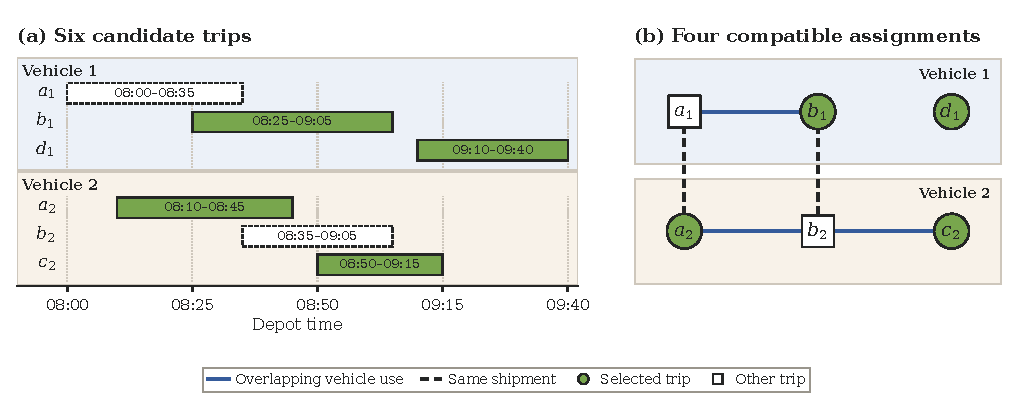
\includegraphics[width=\textwidth]{figures/dispatch_example.pdf}
\caption{\textbf{A four-shipment cold-chain dispatch example.} (a) Each bar spans the loading, travel and turnaround interval of a candidate trip. Letters identify shipments and subscripts identify vehicles. The two bands separate the vehicles. (b) Dashed edges join alternatives for the same shipment. Solid edges join overlapping trips on the same vehicle. The green circles form an independent set, \(\{a_2,b_1,c_2,d_1\}\), that serves all four shipments. The times are illustrative.}
\label{fig:dispatch}
\end{figure*}

Library loading, compilation and checkpoint initialization precede the instance clock. The timer starts with a host edge list and includes construction of the sparse matrix, every solver-specific graph structure, search and publication. OnlineMIS uses the same search code as the timed executable, with an in-memory entry point and callbacks for its greedy solution and best-solution updates. The executable exposes its current node list on exit, while the resident interface retains published improvements during the call. This change affects both setup cost and the set that the caller can access. Clique refinement in our solver publishes upon returning from the native refinement phase. For all three methods, validation of archived sets against the input edges occurs after timing.

We keep the same checkpoint, exchange rules and 3~ms return reserve throughout. For a budget \(B\) in milliseconds, the small and large RB schedules allocate \(\lfloor185B/200\rfloor\) and \(\lfloor175B/200\rfloor\) milliseconds to their respective clique-search phases. The ER schedule uses exchanges throughout. Resident OnlineMIS uses its native iterations until the search deadline. Each independent run begins from the same graph and search seed as its paired controls. We report the wall time at solver completion separately from the time of each archived set.

\paragraph{Controlling for batch throughput on ER.}
In the separate batches, degree search averages 47,807 exchange iterations at 50~ms and 28,255 at 100~ms. We repeat all 12 method--budget combinations within each of the 384 graph--seed blocks on one physical core, with one resident process and GPU. The 12-condition order balances position and immediate predecessor across blocks. Degree search now averages 15,195 iterations at 50~ms and 31,484 at 100~ms, gaining 0.2266 vertices ($[0.1745,0.2839]$). This repeat resolves the reversal in the batched curve. At 200~ms, learned search gains 1.6198 vertices over resident OnlineMIS ($[1.5156,1.7214]$), and 0.0521 over degree search ($[-0.0365,0.1406]$). Each contrast uses a pointwise 95\% interval from graph-level resampling.

\begin{table}[ht]
\centering\small
\caption{Mean feasible set size in the balanced ER repeat. Learned and degree are the two SPRINT-C rankings. All 4,608 runs publish a feasible set before their assigned deadline.}
\label{tab:resident-interleaved}
\begin{tabular}{@{}rrrr@{}}
\toprule
\paperHeader
\paperHead{Budget (ms)} & \paperHead{Learned} & \paperHead{Degree} & \paperHead{OnlineMIS} \\
\midrule
50 & 43.8203 & 43.8828 & 42.2188 \\
100 & 44.1458 & 44.1094 & 42.5443 \\
\rowcolor{TableGold}
200 & 44.3281 & 44.2760 & 42.7083 \\
500 & 44.5521 & 44.5312 & 42.8828 \\
\bottomrule
\end{tabular}
\end{table}


\section{Register interference instances}
\label{app:register}
We include every entry labeled REG in the \href{https://mat.tepper.cmu.edu/COLOR/instances.html}{COLOR instance catalog}: three \texttt{fpsol2}, three \texttt{inithx}, five \texttt{mulsol}, and three \texttt{zeroin} graphs. The \href{https://archive.dimacs.rutgers.edu/pub/challenge/graph/benchmarks/color/}{DIMACS archive} provides the undirected edge lists. We collapse duplicate edges and retain all vertices. The graphs have 184--864 vertices and 10--345 isolated vertices each. All solvers use the same three seeds and a 200~ms cutoff. Both ranking arms use the frozen ER exchange schedule and return reserve. The learned arm uses the same checkpoint as on the RB and ER graphs. All instances are held out of training and schedule selection.

To certify an optimum after the solve, we partition the original vertices into disjoint cliques and verify all within-clique edges. The number of cliques is an upper bound because an independent set can contain at most one vertex per clique. A verified set attains that bound on each of the 14 graphs. Median times to the ultimately optimal set are 0.54~ms for learning, 0.96~ms for degree ranking, and 1.48~ms for OnlineMIS. The two ranking arms execute identical code up to their first delivery. Their median difference therefore measures timing variation before ranking. Mean return times are 197.03, 197.04 and 169.33~ms, respectively. These return times include continued search after the best set has been published.

\section{A worked cold-chain dispatch example}
\label{app:dispatch}
Figure~\ref{fig:dispatch} illustrates the proposed conflict graph on four equal-priority chilled shipments at a single depot. Each candidate is a complete round trip. Its interval includes loading, service, return and vehicle turnaround. Each vehicle can serve one trip at a time. We assume that the listed trips have individually passed temperature, payload and delivery-window checks. The times are illustrative.


There are two kinds of edges. The pairs \((a_1,a_2)\) and \((b_1,b_2)\) duplicate a shipment. The pairs \((a_1,b_1)\), \((a_2,b_2)\), and \((b_2,c_2)\) overlap on a vehicle. The set \(\{a_1,b_2,d_1\}\) is feasible and maximal: every remaining candidate conflicts with a selected assignment. Reassigning A and B gives \(\{a_2,b_1,c_2,d_1\}\), which serves all four shipments. Four is also an upper bound because each shipment can be served only once. This example illustrates both the mapping and the distinction between a maximal decoded set and a maximum set.

\onecolumn
\section{Vertices delivered across scales}
\label{app:cross-scale-witnesses}

We fix the first graph in each released test set (\texttt{idx\_0}) and retain all three benchmark seeds.
On small RB, both priority rules select the same 19 vertices at each seed. Resident OnlineMIS also
delivers 19 vertices each time, but shares only 5, 3 and 5 with SPRINT-C, respectively.
On large RB, the two priority rules each deliver 38 vertices at every seed, with 11, 34 and 22 in
common. On large ER, SPRINT-C delivers 371, 374 and 371 vertices, of which 17, 12 and 13 also
occur in the corresponding OnlineMIS sets. DIMES delivers 286 vertices at 109.2\,ms on the
third seed, its sole timely delivery on this graph. Of these, 29 also belong to the SPRINT-C set.
Full-cohort averages appear in Table~\ref{tab:external-deadline}.

\begin{figure}[!ht]
\centering
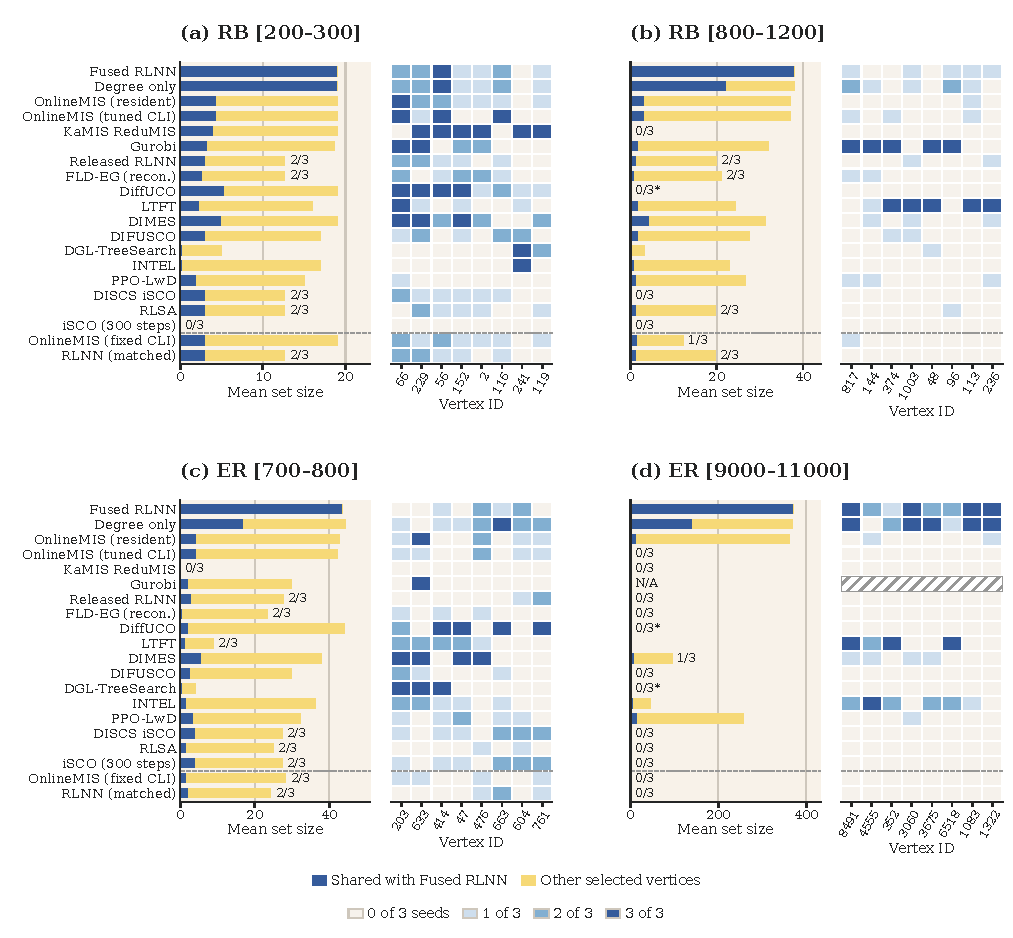
\includegraphics[width=\textwidth]{figures/cross_scale_witnesses.pdf}
\caption{\textbf{Four graphs, with vertex identities preserved across solvers and seeds.}
Each bar is the mean size of the set delivered by 200\,ms over seeds 1017, 1019 and 1021.
Blue counts vertices shared with SPRINT-C at the same seed and yellow counts the remaining
selected vertices. A fraction gives the number of timely deliveries when fewer than three
arrive. An asterisk marks a calibrated solver that skipped search because its predicted runtime
exceeded the budget. Hatching marks the large ER Gurobi model, which exceeds the installed
license limit. Each heatmap shows the eight vertices most frequently selected across the
main-table methods and seeds, ordered by frequency with ties broken by vertex ID. Cell shade
gives the number of seeds on which that solver delivered the vertex. The two rows below the
dashed line are the additional controls from Table~\ref{tab:scale-supplement}.}
\label{fig:cross-scale-witnesses}
\end{figure}


\end{document}
